\newif\ifhandoutmode
% \handoutmodetrue  %comment this line to enable animation

\ifhandoutmode
  \documentclass[handout, aspectratio=169,11pt]{beamer}
\else
  \documentclass[aspectratio=169,11pt]{beamer}
\fi

%──────────────────────────────────────────────────────────────────
%  Theme & colours
%──────────────────────────────────────────────────────────────────
\usetheme{metropolis}
\metroset{sectionpage=none,subsectionpage=none}
\usepackage{appendixnumberbeamer}

\definecolor{DarkBlue}{HTML}{1a1a2e}
\definecolor{MidBlue}{HTML}{16213e}
\definecolor{AccentBlue}{HTML}{0f3460}
\definecolor{AccentPurple}{HTML}{533483}
\definecolor{NeonPink}{HTML}{e94560}
\definecolor{AccentText}{HTML}{FFB8CC}
\definecolor{SoftWhite}{HTML}{f0f0f0}
\definecolor{LightGray}{HTML}{d0d0d0}
\definecolor{Black}{HTML}{000000}

\setbeamercolor{background canvas}{bg=DarkBlue}
\setbeamercolor{normal text}{fg=SoftWhite}
\setbeamercolor{frametitle}{bg=MidBlue,fg=SoftWhite}
\setbeamercolor{title separator}{fg=AccentText}
\setbeamercolor{progress bar}{fg=AccentText,bg=AccentBlue}
\setbeamercolor{block title}{bg=AccentPurple,fg=SoftWhite}
\setbeamercolor{block body}{bg=Black!80,fg=SoftWhite}
\setbeamercolor{alerted text}{fg=AccentText}
\setbeamercolor{itemize item}{fg=AccentText}
\setbeamercolor{itemize subitem}{fg=LightGray}
\setbeamercolor{section in toc}{fg=SoftWhite}

%──────────────────────────────────────────────────────────────────
%  Packages
%──────────────────────────────────────────────────────────────────
\usepackage{tikz}
\usetikzlibrary{arrows.meta,positioning,decorations.pathreplacing,
                shapes.geometric,backgrounds,calc,fit,fadings}
\usepackage{amsmath,amssymb,bm}
\usepackage{booktabs}
\newcommand{\faIcon}[1]{\textbullet}
\usepackage{xcolor}
\usepackage{graphicx}

\usepackage[
  backend=biber,
  style=numeric-comp,
  sorting=none,
  giveninits=true,
  maxbibnames=2,
  doi=false,
  url=false,
  eprint=false,
  isbn=false
]{biblatex}

\addbibresource{references.bib}

%──────────────────────────────────────────────────────────────────
%  Metadata
%──────────────────────────────────────────────────────────────────
\title{\textbf{Diffusion Models}}
\subtitle{How AI Learns to Create Images from Noise}
\author{Presented by: \textit{Anindya, Tamal and Din}}
\date{\today}
\institute{CSE 200: Technical Writing and Presentation\\\textbf{Bangladesh University of Engineering and Technology}}

%──────────────────────────────────────────────────────────────────
%  Custom commands
%──────────────────────────────────────────────────────────────────
\newcommand{\highlight}[1]{\textcolor{AccentText}{\textbf{#1}}}
\newcommand{\soft}[1]{\textcolor{LightGray}{#1}}

\hypersetup{
  bookmarksopen=true,
  bookmarksnumbered=true,
  pdfauthor={Anindya, Tamal and Din},
  pdftitle={Diffusion Models: How AI Learns to Create Images from Noise},
}

%══════════════════════════════════════════════════════════════════
\begin{document}
%══════════════════════════════════════════════════════════════════

%──────────────────────────────────────────────────────────────────
% TITLE SLIDE
%──────────────────────────────────────────────────────────────────
{
\setbeamercolor{background canvas}{bg=DarkBlue}

\begin{frame}[plain]
  \begin{tikzpicture}[remember picture,overlay]
    \foreach \r/\op in {5/0.05,3.5/0.08,2/0.12}{
      \fill[NeonPink,opacity=\op]
      (current page.north east) circle (\r cm);
      }
      \foreach \r/\op in {4/0.05,2.5/0.08,1.2/0.12}{
        \fill[AccentPurple,opacity=\op]
        (current page.south west) circle (\r cm);
        }
      \end{tikzpicture}
      \vspace{1.4cm}
      \titlepage
    \end{frame}
}

\begin{frame}{Outline}
  \tableofcontents
\end{frame}

%══════════════════════════════════════════════════════════════════
% SLIDE 1 — What Problem Are We Solving?
%══════════════════════════════════════════════════════════════════

\section{Introduction}

\begin{frame}{What Problem Are We Solving?}
  \vspace{4pt}
  \begin{figure}
    \centering
    \begin{minipage}[c]{\linewidth}
      \centering
      \begin{minipage}[b]{0.2\linewidth}
        \centering
        \includegraphics[width=\linewidth]{images/Real_Face.png}
        \\[1pt]
        {\tiny Real face}
      \end{minipage}
      \hspace{0.2\linewidth}
      \begin{minipage}[b]{0.2\linewidth}
        \centering
        \includegraphics[width=\linewidth]{images/AI_Generated_Face_05.png}
        \\[1pt]
        {\tiny AI-generated face \textit{(Sora)}}
      \end{minipage}
    \end{minipage}
  \end{figure}

  \pause
  \vspace{4pt}
  \begin{block}{Generative Modeling}
    Can a machine learn to \highlight{create new, realistic samples}
    that are indistinguishable from real data?
  \end{block}
  \pause
  \begin{center}
    \highlight{Diffusion models} provide a stable, high-quality solution.
  \end{center}
\end{frame}

%══════════════════════════════════════════════════════════════════
% SLIDE 2 — The Core Idea: Learning by Destroying
%══════════════════════════════════════════════════════════════════
\section{Core Idea}

\begin{frame}{The Core Idea: Learning by Destroying}

  \begin{center}
    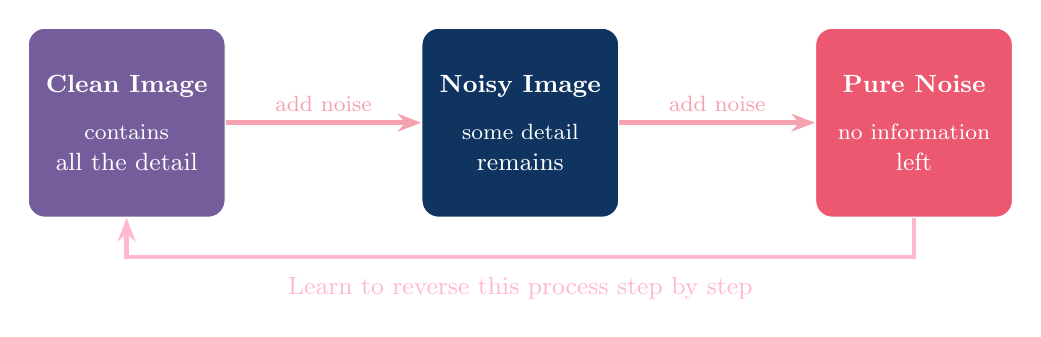
\begin{tikzpicture}[
      stage/.style={rounded corners=6pt, draw=white!30,
                    minimum width=2.5cm, minimum height=2.4cm,
                    font=\small, text=white, align=center,
                    inner sep=6pt},
      bigarr/.style={-{Stealth[length=3mm]}, line width=1.6pt}]

      %% Forward (destroy)
      \node<1->[stage, fill=AccentPurple!80] (clean) at (0,0)
        {\textbf{Clean Image}\\[6pt]\footnotesize contains\\all the detail};
      \node<2->[stage, fill=AccentBlue] (mid) at (5,0)
        {\textbf{Noisy Image}\\[6pt]\footnotesize some detail\\remains};
      \draw<2->[bigarr, NeonPink!50] (clean) -- (mid)
        node[midway, above, font=\footnotesize]{add noise};
      \node<3->[stage, fill=NeonPink!90] (noise) at (10,0)
        {\textbf{Pure Noise}\\[6pt]\footnotesize no information\\left};
      \draw<3->[bigarr, NeonPink!50] (mid) -- (noise)
        node[midway, above, font=\footnotesize]{add noise};
      %% Reverse (learn)
      \draw<4->[bigarr, AccentText] (noise.south) -- ++(0,-0.5) -| (clean.south);
      \node<4->[font=\small, text=AccentText, align=center] at (5,-2.1)
        {Learn to reverse this process step by step};

    \end{tikzpicture}
    \pause[5]

    \vspace{6pt}
    
    \begin{block}{We Essentially Have Two Diffusion Processes}
      \begin{itemize}
        \item The \textbf{Forward Diffusion Process} that gradually adds noise.\\
        \item The \textbf{Reverse Diffusion Process} that removes noise step by step.\\
      \end{itemize}
    \end{block}
  \end{center}
\end{frame}

%══════════════════════════════════════════════════════════════════
% SLIDE 3 — The Forward Process: Adding Noise
%══════════════════════════════════════════════════════════════════
\section{Forward Diffusion Process}
\begin{frame}{The Forward Diffusion Process: Adding Noise}

  \vspace{10pt}
  \begin{center}
    \begin{minipage}{0.22\linewidth}
      \centering
      \includegraphics[height=3.0cm,keepaspectratio]{images/clean.png}\\[2pt]
      {\scriptsize Clean Image}
    \end{minipage}
    \pause
    \hfill
    \begin{minipage}{0.22\linewidth}
      \centering
      \includegraphics[height=3.0cm,keepaspectratio]{images/noised_slightly.png}\\[2pt]
      {\scriptsize Slightly Noisy}
    \end{minipage}
    \pause
    \hfill
    \begin{minipage}{0.22\linewidth}
      \centering
      \includegraphics[height=3.0cm,keepaspectratio]{images/noised_heavily.png}\\[2pt]
      {\scriptsize Heavily Noisy}
    \end{minipage}
    \pause
    \hfill
    \begin{minipage}{0.22\linewidth}
      \centering
      \includegraphics[height=3.0cm,keepaspectratio]{images/noised_fully.png}\\[2pt]
      {\scriptsize Pure Noise}
    \end{minipage}
  \end{center}
  \pause

  \begin{block}{What Happens}
    Take a real image and add a \emph{tiny} bit of random noise.
    Repeat this hundreds of times until only noise remains.
  \end{block}
\end{frame}

%══════════════════════════════════════════════════════════════════
% SLIDE 4 — The Reverse Process: Removing Noise
%══════════════════════════════════════════════════════════════════
\section{Reverse Diffusion Process}
\begin{frame}{The Reverse Diffusion Process: Removing Noise}

  \vspace{10pt}
  \begin{center}
    \begin{minipage}{0.22\linewidth}
      \centering
      \includegraphics[height=3.0cm,keepaspectratio]{images/noised_fully.png}\\[2pt]
      {\scriptsize Pure Noise}
    \end{minipage}
    \pause
    \hfill
    \begin{minipage}{0.22\linewidth}
      \centering
      \includegraphics[height=3.0cm,keepaspectratio]{images/noised_heavily.png}\\[2pt]
      {\scriptsize Slightly Less Noisy}
    \end{minipage}
    \pause
    \hfill
    \begin{minipage}{0.22\linewidth}
      \centering
      \includegraphics[height=3.0cm,keepaspectratio]{images/noised_slightly.png}\\[2pt]
      {\scriptsize Almost Denoised}
    \end{minipage}
    \pause
    \hfill
    \begin{minipage}{0.22\linewidth}
      \centering
      \includegraphics[height=3.0cm,keepaspectratio]{images/clean.png}\\[2pt]
      {\scriptsize Fully Denoised}
    \end{minipage}
  \end{center}
  \pause

  \begin{block}{How Generation Works}
    \begin{itemize}
      \item Start from \highlight{pure noise}
      \item Predict and remove a little noise at each step
      \item Repeat until a realistic image appears
    \end{itemize}
  \end{block}
\end{frame}

\section{Training}
\begin{frame}{Training}
  \begin{center}
    {To produce realistic images, the model must learn to reverse the noise process.}\\[20pt]
    \pause
    {\setlength{\fboxsep}{8pt}\colorbox{AccentBlue}{\Large \highlight{But how does the model learn this reverse process?}}}
  \end{center}
\end{frame}

%══════════════════════════════════════════════════════════════════
% SLIDE 5 — How Do We Train It?
%══════════════════════════════════════════════════════════════════
\begin{frame}{How Do We Train It?}

  \begin{center}
    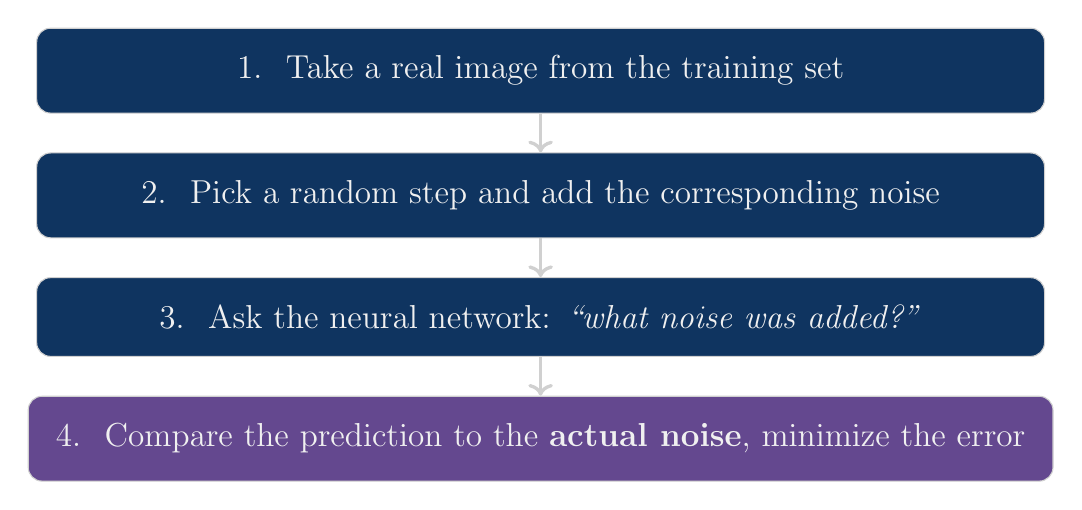
\begin{tikzpicture}[
      trainstep/.style={rounded corners=5pt, draw=LightGray,
                   fill=AccentBlue, text=SoftWhite,
                   minimum width=12.8cm, minimum height=1.0cm,
                   font=\large, inner sep=10pt, align=left},
      arr/.style={->, LightGray, line width=1.2pt}]

      \node<1->[trainstep] (s1) at (0,0)
        {1.\; Take a real image from the training set};
      % \pause
      \node<2->[trainstep, below=14pt of s1] (s2)
        {2.\; Pick a random step and add the corresponding noise};
      \draw<2->[arr] (s1.south) -- (s2.north);
      % \pause
      \node<3->[trainstep, below=14pt of s2] (s3)
        {3.\; Ask the neural network: \textit{``what noise was added?''}};
      \draw<3->[arr] (s2.south) -- (s3.north);
      % \pause
      \node<4->[trainstep, below=14pt of s3, fill=AccentPurple!90] (s4)
        {4.\; Compare the prediction to the \textbf{actual noise}, minimize the error};
      \draw<4->[arr] (s3.south) -- (s4.north);

      % \foreach \a/\b in {s1/s2, s2/s3, s3/s4}
      %   \draw[arr] (\a.south) -- (\b.north);
    \end{tikzpicture}
  \end{center}
\end{frame}

\section{Insights}
\begin{frame}{Key Insight \& Why It Works}
  \begin{columns}[T]
    \column{0.48\textwidth}
      \begin{block}{Key Insight}
        \begin{itemize}
          \item We add \textbf{known} noise
          \item So we have exact labels
          \item Training target is clear and reliable
        \end{itemize}
      \end{block}

    \column{0.48\textwidth}
      \begin{block}{Why It Works}
        \begin{itemize}
          \item Model learns many small denoising steps
          \item Small steps are easier to learn
          \item Chaining them builds a full image
        \end{itemize}
      \end{block}
  \end{columns}
\end{frame}

%══════════════════════════════════════════════════════════════════
% SLIDE 6 — Why Diffusion Models Work So Well
%══════════════════════════════════════════════════════════════════

\begin{frame}{Why Diffusion Models Work So Well}
  \begin{block}{Advantages}
    \begin{itemize}
      \item \highlight{Stable training}
      \item \highlight{High Quality Samples}
      \item \highlight{Good Diversity} {\small (less mode collapse than GANs)}
      \item \highlight{Flexible Conditioning} {\small (text-to-image, video-generation, audio synthesis)}
      \item \highlight{Strong Theoretical Foundation}
    \end{itemize}
  \end{block}

  \vspace{6pt}
  \begin{center}
    \soft{In practice, diffusion models combine reliability with strong output quality.}
  \end{center}
\end{frame}

\begin{frame}{Summary}
  \begin{center}
    \Large
    \highlight{Diffusion models generate \textit{data} by learning to reverse a gradual noise process.}
  \end{center}
\end{frame}

%══════════════════════════════════════════════════════════════════
% SLIDE 7 — Applications
%══════════════════════════════════════════════════════════════════
\section{Applications}
\begin{frame}{Applications}
  \vspace{6pt}
  \begin{center}
    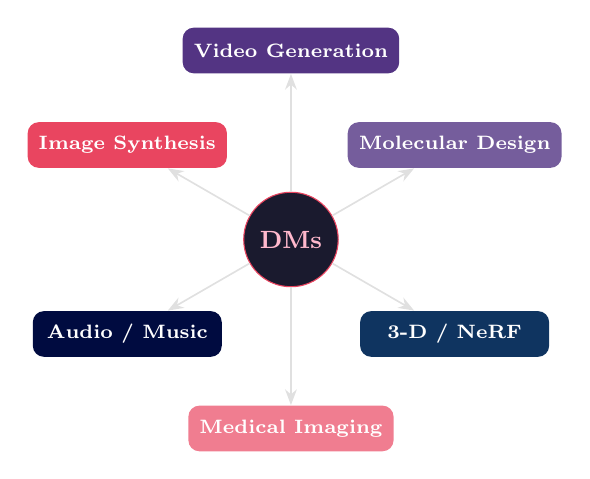
\begin{tikzpicture}[
      app/.style={rounded corners=4pt,
                  minimum width=2.4cm, minimum height=0.58cm,
                  font=\scriptsize\bfseries, text=white,
                  inner sep=4pt, align=center},
      apparrow/.style={-{Stealth[length=2mm]},
                       LightGray!65, line width=0.6pt},
      every node/.style={font=\scriptsize}]

      \node[draw=NeonPink, circle, fill=DarkBlue,
            font=\small\bfseries, text=AccentText,
            minimum size=1.2cm] (c) at (0,0) {DMs};

      \node[app, fill=NeonPink]        (img)   at (150:2.4cm) {Image Synthesis};
      \node[app, fill=AccentBlue!120]  (aud)   at (210:2.4cm) {Audio / Music};
      \node[app, fill=NeonPink!70]     (med)   at (270:2.4cm) {Medical Imaging};
      \node[app, fill=AccentBlue]      (threed)at (330:2.4cm) {3-D / NeRF};
      \node[app, fill=AccentPurple!80] (mol)   at ( 30:2.4cm) {Molecular Design};
      \node[app, fill=AccentPurple]    (vid)   at ( 90:2.4cm) {Video Generation};

      \foreach \dest in {img, aud, med, threed, mol, vid}
        \draw[apparrow] (c) -- (\dest);
    \end{tikzpicture}
  \end{center}
\end{frame}

\begin{frame}{Some Real-World Tools Powered by Diffusion}
  \begin{center}
    \begin{minipage}{0.36\textwidth}
      \centering
      \includegraphics[height=2cm]{images/Midjourney-White-Logo-PNG.png}\\[5pt]
      {\small \highlight{Midjourney}}
    \end{minipage}
    \pause
    \vspace{8pt}

    \begin{minipage}{0.36\textwidth}
      \centering
      \includegraphics[height=1.05cm]{images/white-dall-e-logo-png.png}\\[5pt]
      \vspace{13pt}
      {\small \highlight{DALL·E}}
    \end{minipage}
    \pause
    \hspace{0.08\textwidth}
    \begin{minipage}{0.36\textwidth}
      \vspace{6pt}
      \centering
      \includegraphics[height=1.5cm]{images/Open-AI-Sora-White-Logo-PNG.png}\\[4pt]
      {\small \highlight{OpenAI Sora}}
    \end{minipage}
  \end{center}
\end{frame}

%══════════════════════════════════════════════════════════════════
% SLIDE 8 — Limitations & Open Challenges
%══════════════════════════════════════════════════════════════════
\section{Limitations \& Challenges}
\begin{frame}{Limitations \& Open Challenges}
  \begin{columns}[T]
    \column{0.50\textwidth}
      \begin{block}{Current Limitations}
        \begin{itemize}
          \item \textbf{Slow generation} — requires many denoising steps
                (hundreds to thousands)
          \item \textbf{High compute cost} — training requires significant
                GPU resources
          \item \textbf{Large model size} — not easy to run on consumer hardware
        \end{itemize}
      \end{block}

    \column{0.47\textwidth}
      \begin{block}{Open Questions}
        \begin{itemize}
          \item Can we make generation \highlight{faster}?
                (Active research area)
          \item How do we ensure generated content is \highlight{safe and ethical}?
          \item Can we extend to \highlight{longer videos} and
                \highlight{interactive content}?
        \end{itemize}
      \end{block}
  \end{columns}
\end{frame}

%──────────────────────────────────────────────────────────────────
% THANK YOU SLIDE
%──────────────────────────────────────────────────────────────────
\setbeamercolor{background canvas}{bg=DarkBlue}

\section{Conclusion}

\begin{frame}
  \begin{tikzpicture}[remember picture,overlay]
    \foreach \r/\op in {6/0.04,4/0.07,2.2/0.11}{
      \fill[NeonPink,opacity=\op]
        (current page.center) circle (\r cm);
    }
  \end{tikzpicture}
  % \vspace{1.2cm}
  \begin{center}
    {\Huge\bfseries\color{SoftWhite} Thank You!}\\[10pt]
    {\large\color{LightGray} Thanks for Listening!}
  \end{center}
\end{frame}

%──────────────────────────────────────────────────────────────────
% REFERENCES SLIDE
%──────────────────────────────────────────────────────────────────
\begin{frame}{References}
  \footnotesize
  \setlength{\bibitemsep}{4pt}
  \nocite{ho2020ddpm,song2019generative,song2020denoising,nichol2021improved}
  \printbibliography[heading=none]
\end{frame}

\end{document}